\documentclass[titlepage, 12pt, oneside]{article}

\usepackage[dvipsnames,table]{xcolor} 

\definecolor{Gray}{gray}{0.5}
\definecolor{linkblue}{HTML}{0A3D5C}
\definecolor{darkgreen}{HTML}{2E7D32}

\usepackage{float}

\usepackage{hyphenat}

\usepackage{setspace}

\linespread{1.5}

\usepackage[english]{babel}

\usepackage{mathtools}
\usepackage{amsmath}

\usepackage{caption}

\usepackage[T1]{fontenc}

\usepackage{lmodern}

\usepackage{newtxtext,newtxmath}

\usepackage{enumerate}

\usepackage{enumitem}

\usepackage{etoolbox}
\AtBeginEnvironment{thebibliography}{\setlength{\leftskip}{0pt}\setlength{\itemindent}{0pt}}

\setlist[itemize]{leftmargin=*}

\usepackage{graphicx}
\graphicspath{{figures/}}

\usepackage[a4paper, top=2.5cm, bottom=2.5cm, left=3cm, right=2.5cm]{geometry}

\usepackage{fancyhdr, ifthen}
\pagestyle{fancy}
\fancyhf{}
\lhead{Exploring South African Crime Trends}
\rhead{Page \thepage}

\renewcommand{\headrulewidth}{0.5pt}
\renewcommand{\footrulewidth}{0.5pt}

\fancyheadoffset[R]{0pt}

\usepackage{xurl}

\usepackage[breaklinks,linktocpage=true]{hyperref}

\hypersetup{colorlinks=true,
	urlcolor=linkblue,
	citecolor=linkblue,
	linkcolor=darkgreen,
	pageanchor=false}

\urlstyle{same}

\usepackage[nameinlink]{cleveref}

\usepackage{multirow}

\usepackage{booktabs}

\usepackage{array}

\usepackage{eso-pic}

\usepackage{subcaption}

\usepackage{appendix}

\usepackage{adjustbox}

\usepackage{pdflscape}

\usepackage[most]{tcolorbox}

\usepackage{tabularx}
\newcolumntype{Y}{>{\centering\arraybackslash}X}

\makeatletter
\AtBeginDocument{\renewcommand{\bibname}{References}}
\renewcommand\@biblabel[1]{}
\renewenvironment{thebibliography}[1]
{\phantomsection\section*{\refname}%
	\@mkboth{\MakeUppercase\refname}{\MakeUppercase\refname}%
	\renewcommand{\bibname}{References}
	\list{}%
	{\leftmargin0pt
		\itemindent0pt
		\labelwidth0pt
		\labelsep0pt
		\@openbib@code
		\usecounter{enumiv}}%
	\sloppy
	\clubpenalty4000
	\@clubpenalty \clubpenalty
	\widowpenalty4000%
	\sfcode`\.\@m}
{\def\@noitemerr
	{\@latex@warning{Empty `thebibliography' environment}}%
	\endlist}
\makeatother

\usepackage[nottoc]{tocbibind}

\usepackage[titles]{tocloft}

\setlength{\cftfigindent}{0pt}

\usepackage{titlesec}

\usepackage{microtype}

\hypersetup{pdfstartview={XYZ null null null}}

\begin{document}

\begin{titlepage}
{\centering

\textcolor[HTML]{2E7D32}{\rule{0.8\linewidth}{1pt}}

\vspace{0.15cm}

{\Huge \textbf{Exploring South African\\[0.3cm] Crime Trends}}

\vspace{0.35cm}

{\Large \textbf{\textcolor[HTML]{2E7D32}{A Data-Driven Analysis (2011--2023)}}}

\vspace{0.35cm}

{\large An Exploratory Data Analysis Summary}

\textcolor[HTML]{2E7D32}{\rule{0.8\linewidth}{1pt}}

\vspace{0.5cm}

{\large Prepared by}

\vspace{0.25cm}

{\Large \textbf{Joshua Pillay}}

\vspace{0.75cm}

{\large \textcolor[HTML]{2E7D32}{\textbf{Tools Used:}}}\\[0.03cm] 
{\large Excel $\bullet$ Python $\bullet$ MATLAB $\bullet$ SQL $\bullet$ Power BI}

\vspace{0.45cm}

{\large \textcolor[HTML]{2E7D32}{\textbf{Repository:}}}\\[0.03cm] 
{\large \url{https://github.com/joshua-pillay/sa-crime-statistics}}

\vspace{0.45cm}

{\large May 2026}

\vspace{0.25cm}}

\subsection*{\centering Abstract}
\noindent This summary presents an exploratory, spatial, and predictive analysis of South African Police Service crime statistics spanning 12 years across nine provinces and seven crime categories. The analysis of crime statistics is a necessity for supporting existing frameworks in an effort to address the current South African crimescape. A multi-tool pipeline spanning Excel, Python, SQL, MATLAB and Power BI was used for EDA, geospatial analysis, trend decomposition, and time series forecasting. The analysis revealed the dominating provinces and their associated geographic crime concentration, the prevalent crime categories and the annual national crime patterns across the full analysis period. Near-term forecasting revealed no likely decline in projected figures without structural intervention. The analysis and its findings may support existing frameworks by potentially informing a data-driven approach to address South Africa's crime burden.


\end{titlepage}

\section*{Introduction \& Methodology}

Crime is regarded as a national priority in South Africa and, as such, remains one of the most significant challenges to the country’s economic development
and social stability. South Africa’s governance response to its crime burden is formalised through several strategic frameworks, emphasising the relevance of structured, evidence-based analysis of SAPS crime statistics to national policing priorities. The analytically-rich nature of the published multi-year SAPS crime statistics favours an in-depth analysis of the national and provincial crime figures to potientially support a data-driven approach that addresses South Africa's crime burden. The analysis was conducted to better understand the nature of crime in South Africa from temporal, spatial, and categorical perspectives, addressing four research questions. Particular attention is paid to the influence of anomalous periods (COVID-19) on reported crime figures.\\\\
The dataset was publicly sourced from Kaggle, with the raw dataset comprising  (9 provinces + 1 national) $\times$ 7 crime categories $\times$ 12 financial years = 840 row entries. The data analysis was conducted across eight stages, with each stage implementing a designated tool in a distinct, non-overlapping role within the analytical pipeline (\Cref{analytical_pipeline}). Upon assessing the data quality in Stage 1, national row entries were then filtered, reducing total rows entries to 9 provinces $\times$ 7 crime categories $\times$ 12 financial years = 756. Additionally, Two discrepancies in crime figures were also addressed. Stage 2 comprised several data cleaning steps: renaming column labels, province entries, category entries, and parsing year entries to 4-character integers. 

\vspace{\fill}

\begin{table}[H]
	\centering
	\caption{Analytical pipeline.}
	\begin{tabularx}{\linewidth}{llX}
		\toprule
		\textbf{Stage} & \textbf{Tool} & \textbf{Purpose} \\
		\midrule
		 1 & Excel & Data profiling and transformation \\[0.3cm]
		 2 & Python & Data cleaning and preparation \\[0.3cm]
		 3 & Python & Exploratory data analysis \\[0.3cm]
		 4 & Python & Geospatial analysis \\[0.3cm]
		 5 & MATLAB & Trend decomposition \\[0.3cm]
		 6 & Python & Time series forecasting \\[0.3cm]
		 7 & SQL & Structured querying for cross-validation \\[0.3cm]
		 8 & Power BI & Interactive dashboard  \\
		\bottomrule
	\end{tabularx}
	\label{analytical_pipeline}
\end{table}

\newpage

\section*{EDA \& Spatial Analysis}

\vspace{\fill}

\begin{figure}[H]
	\centering
	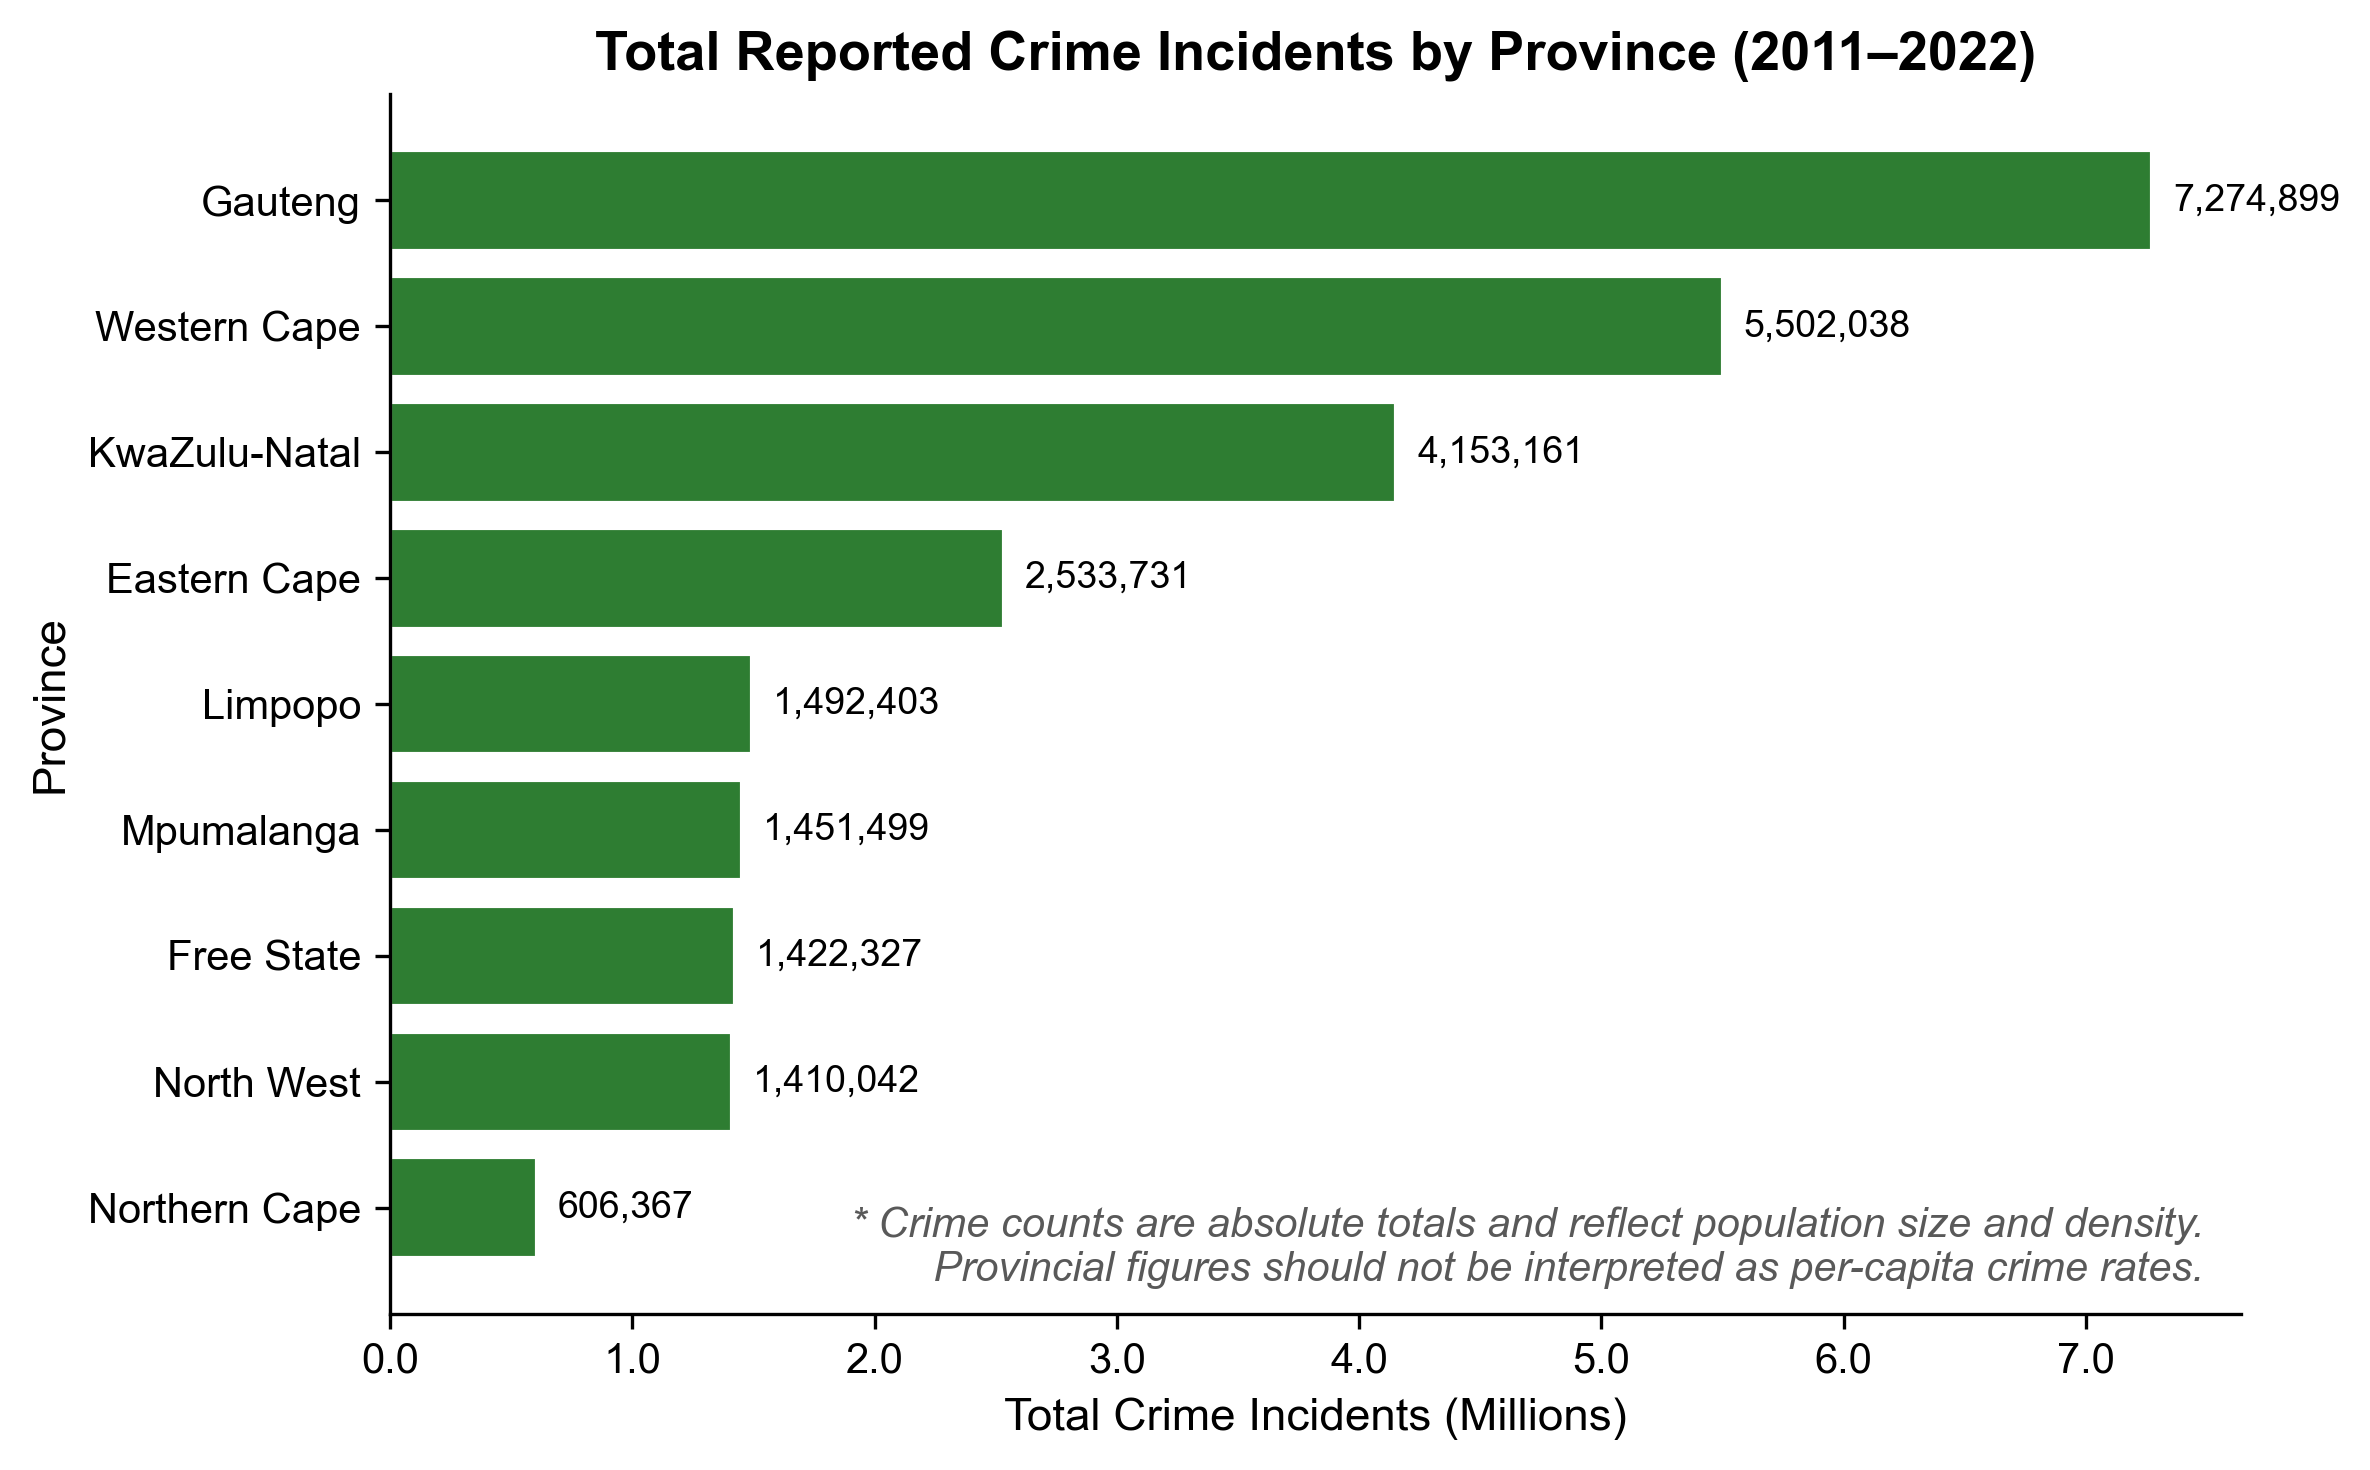
\includegraphics[width=0.925\linewidth]{province_bar_chart.png}
	\caption{Total reported crimes by province (2011 -- 2022).}
	\label{fig:province_bar}
\end{figure}

\vspace{\fill}

\begin{figure}[H]
	\centering
	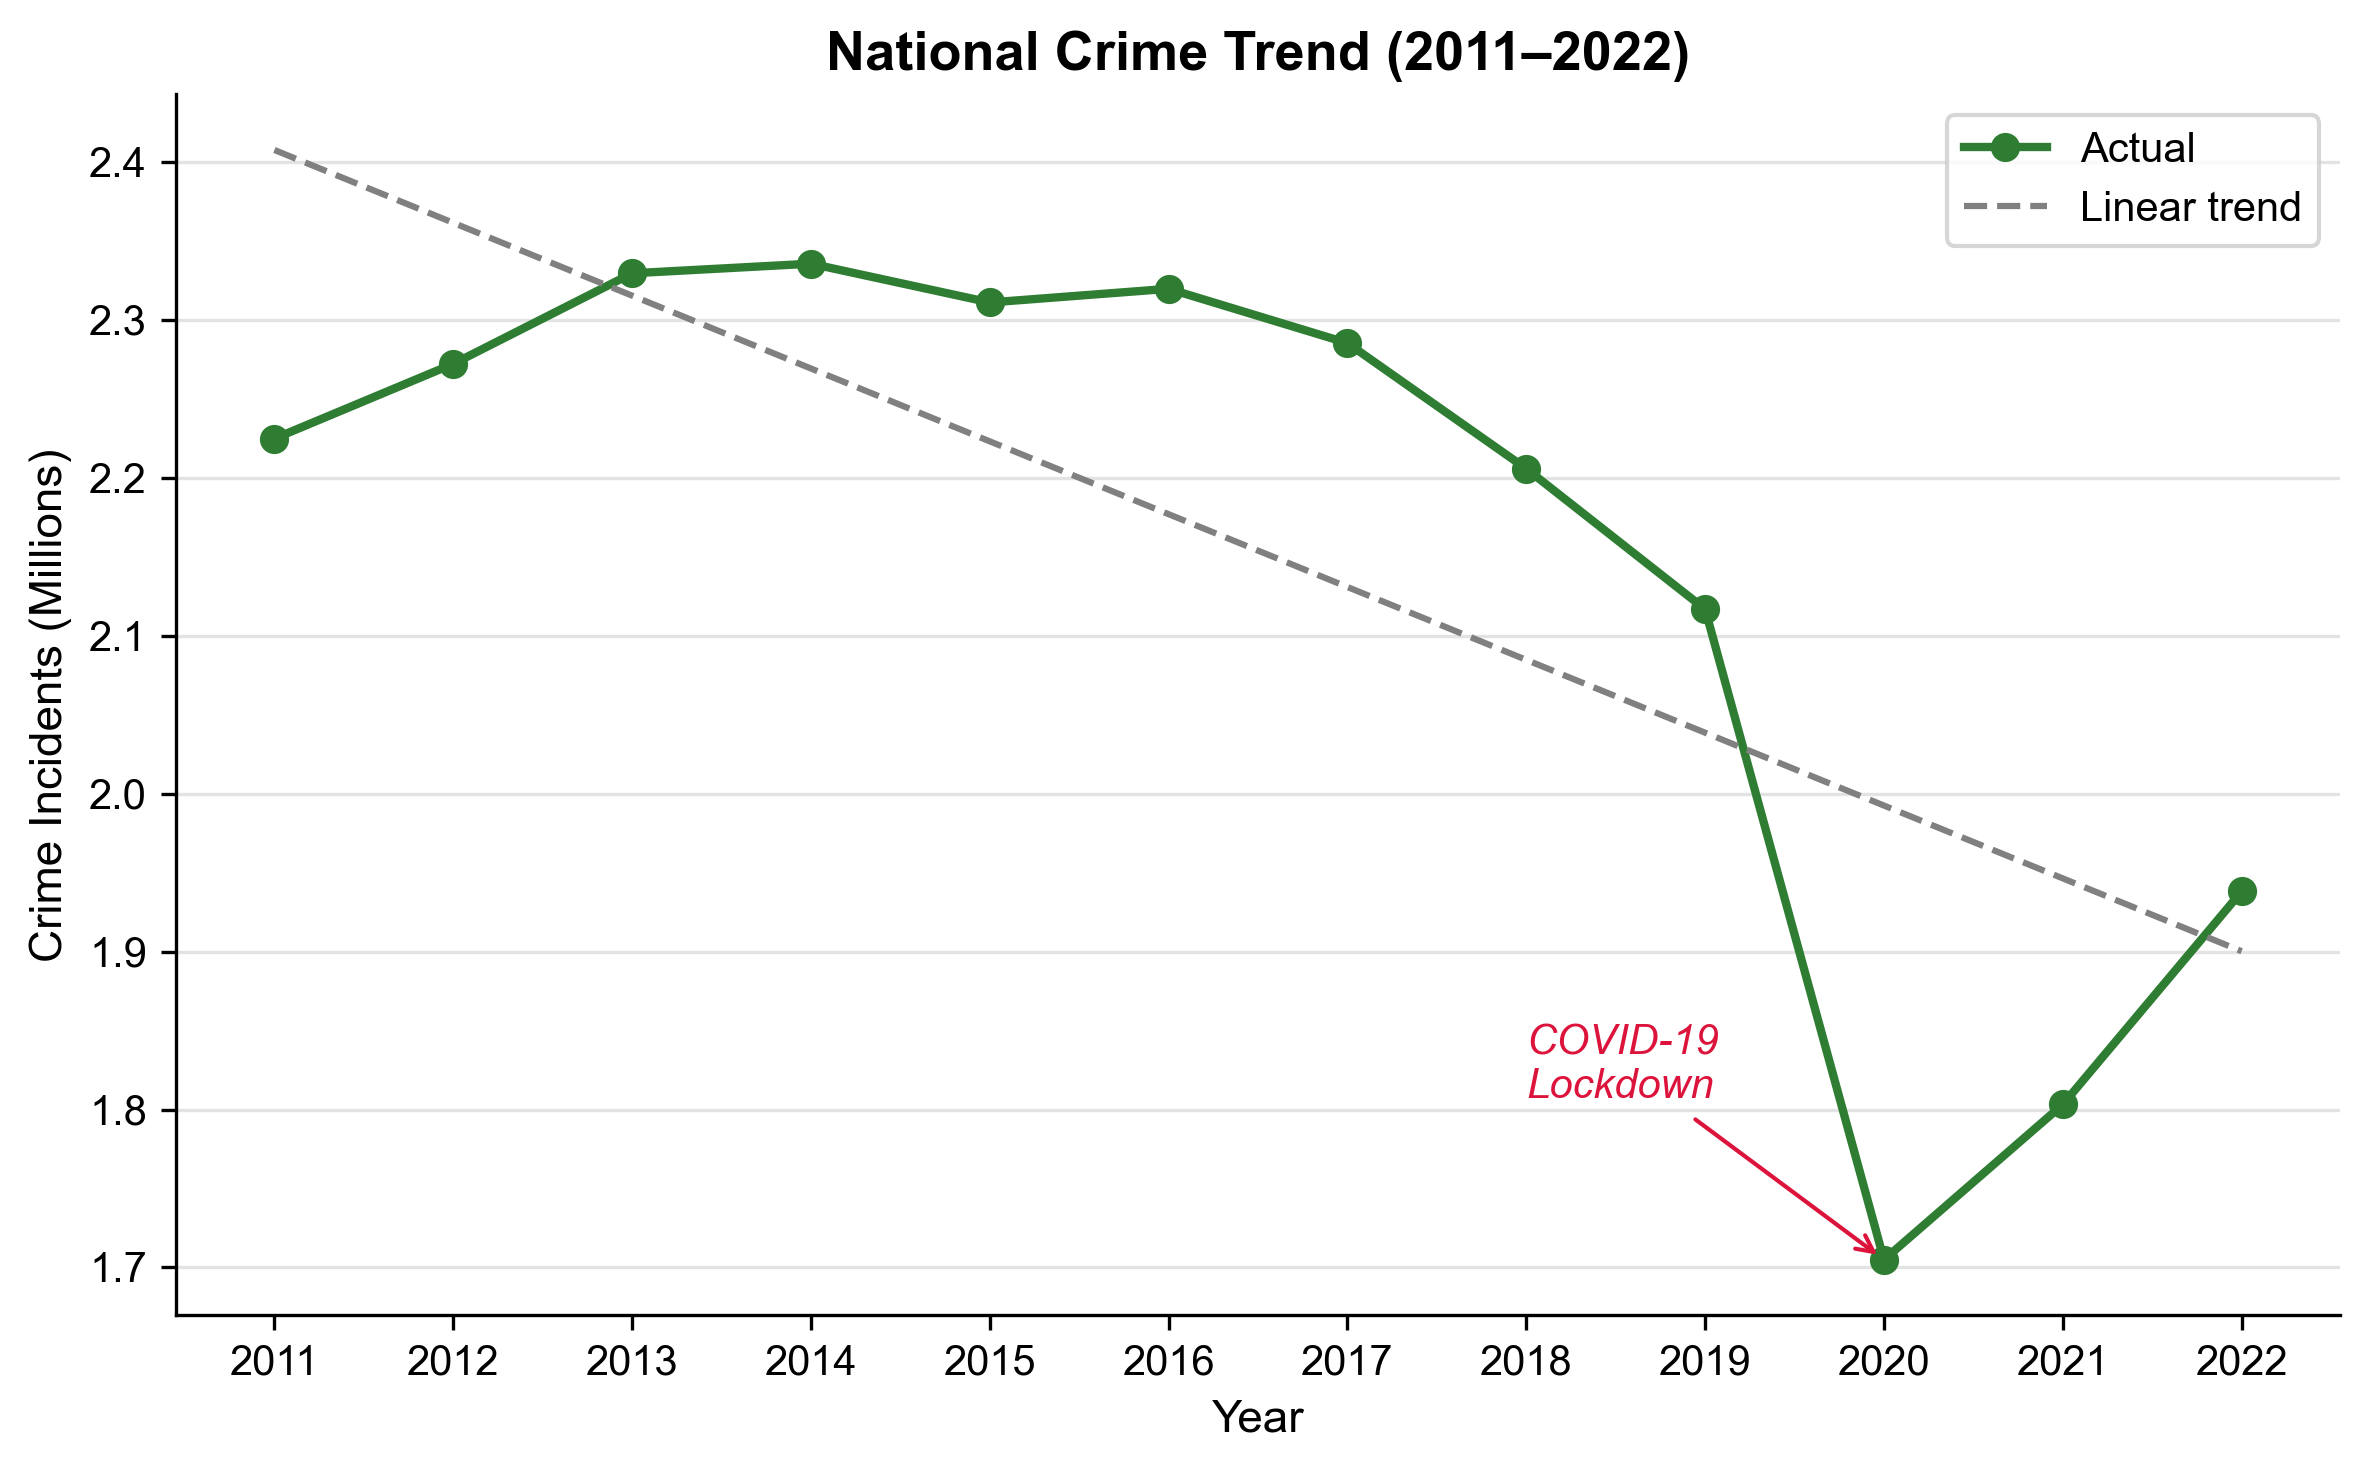
\includegraphics[width=0.925\linewidth]{national_crime_trend.png}
	\caption{National crime trend with COVID-19 annotation (2011 -- 2022).}
	\label{fig:national_trend}
\end{figure}

\vspace{\fill}

\newpage

\begin{figure}[H]
	\centering
	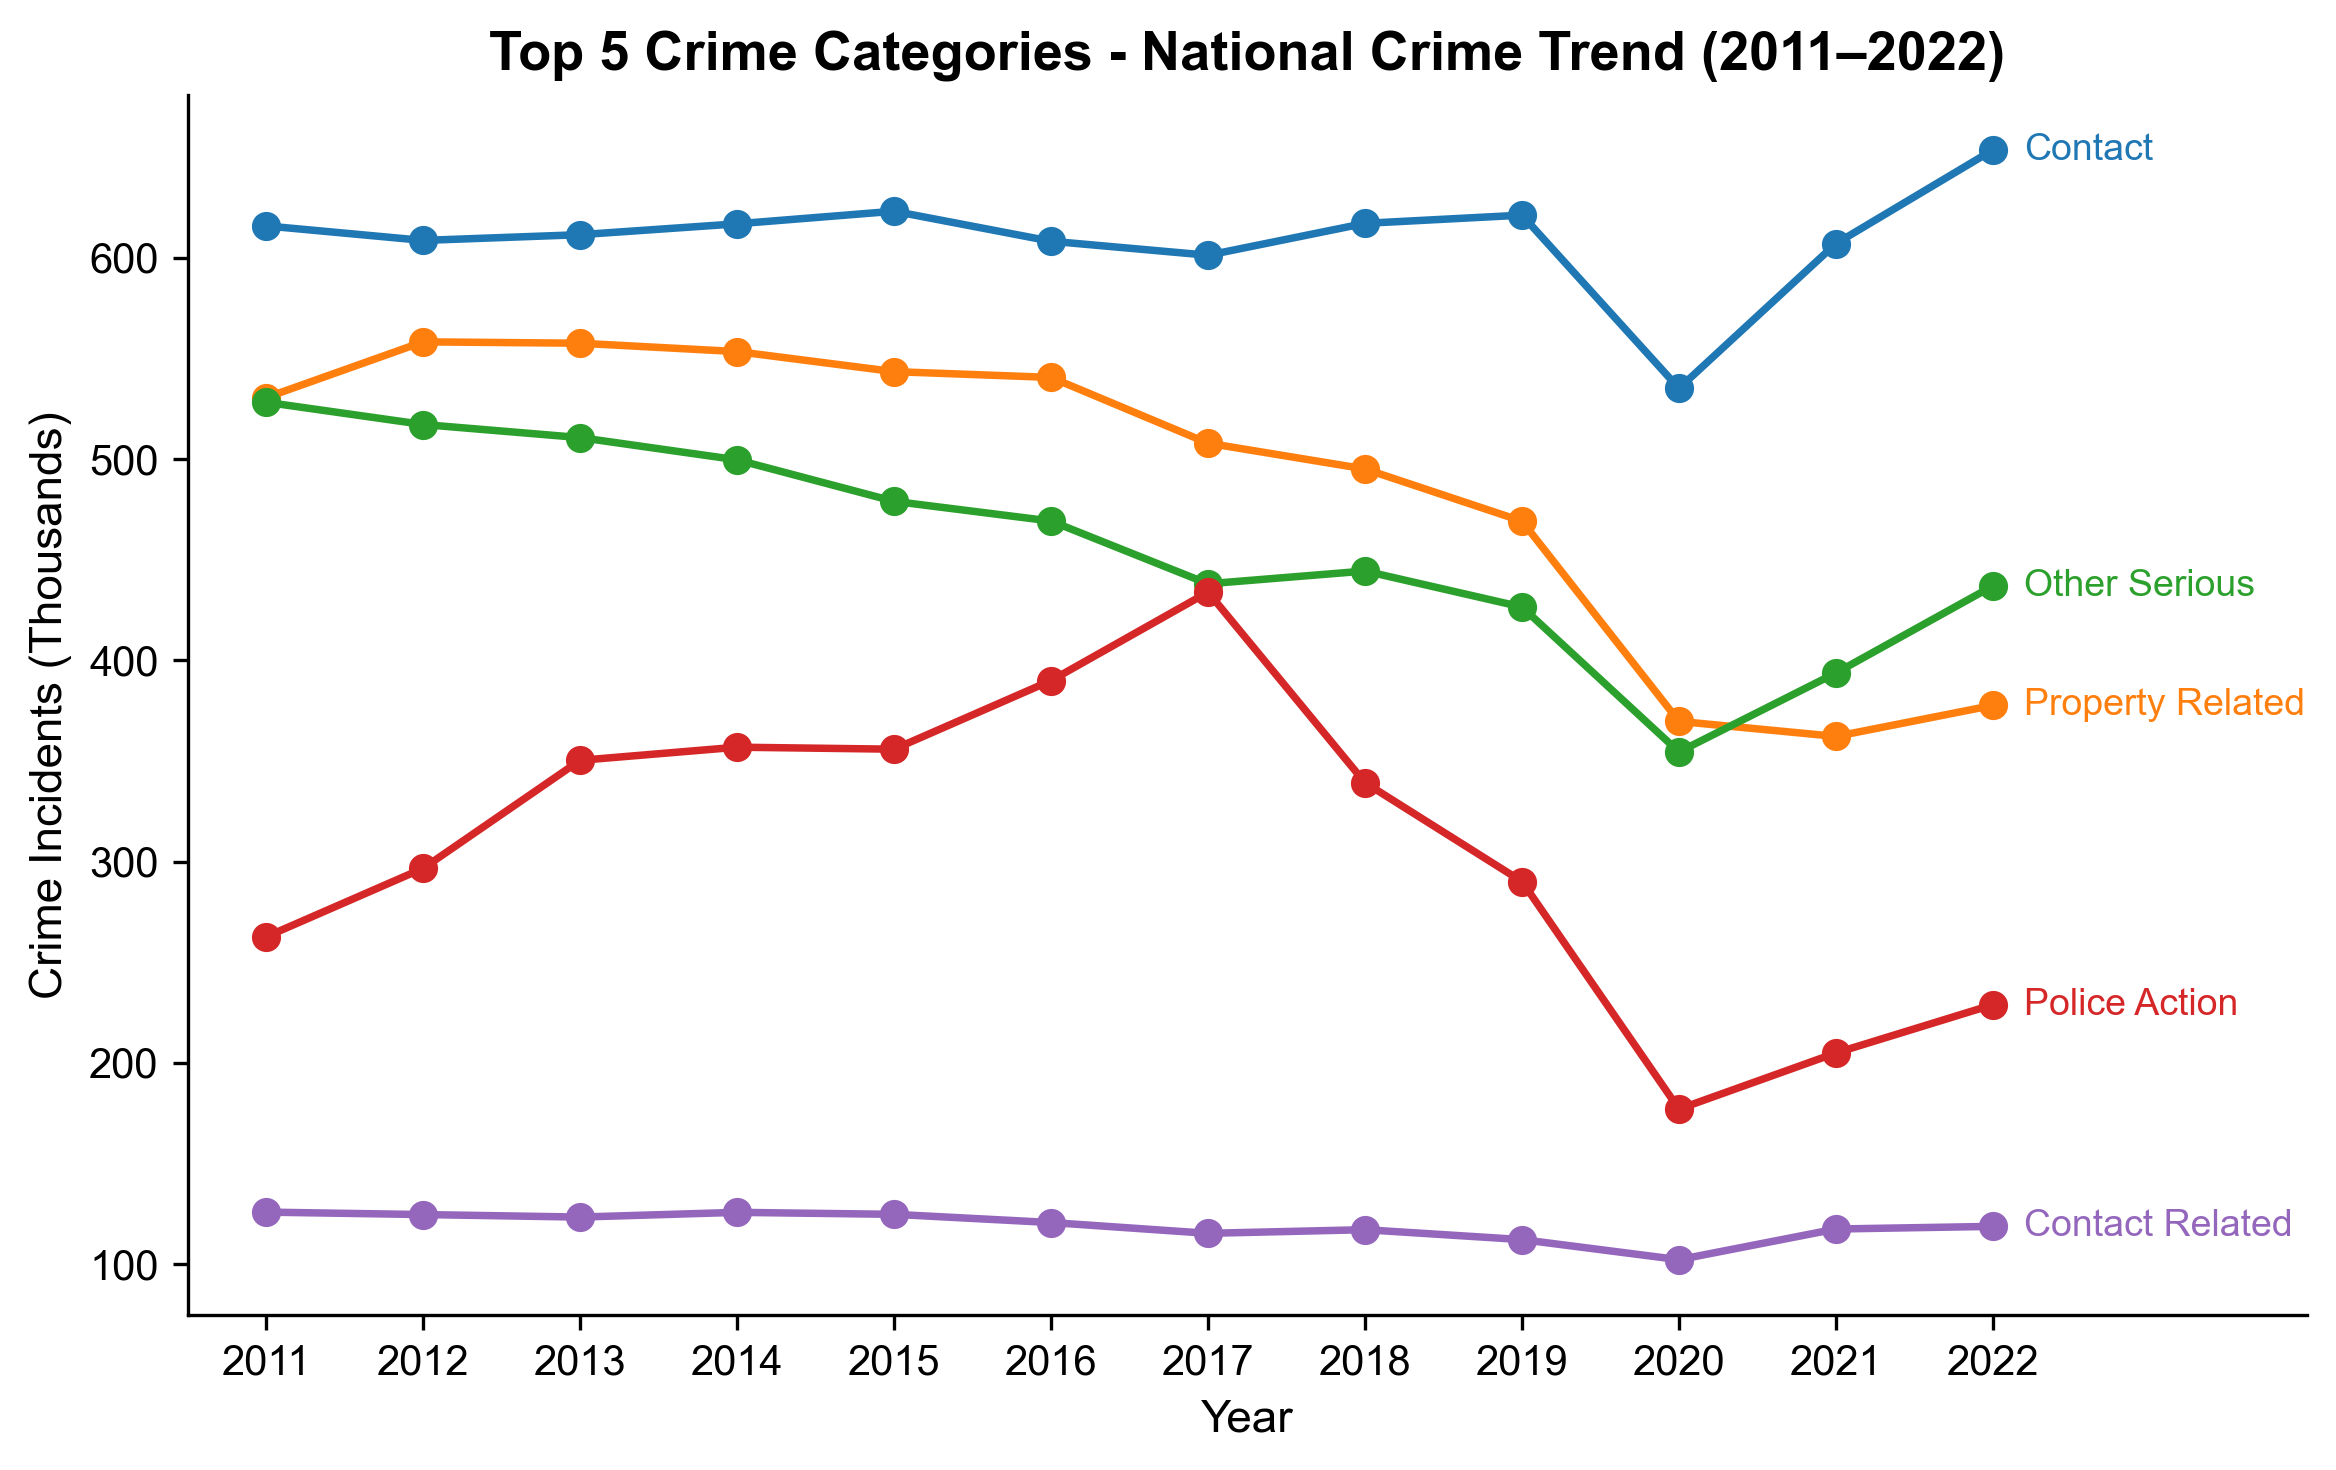
\includegraphics[width=0.835\linewidth]{top5_categories.png}
	\caption{National trend of top 5 crime categories (2011 -- 2022).}
	\label{fig:top5}
\end{figure}

\begin{figure}[H]
	\centering
	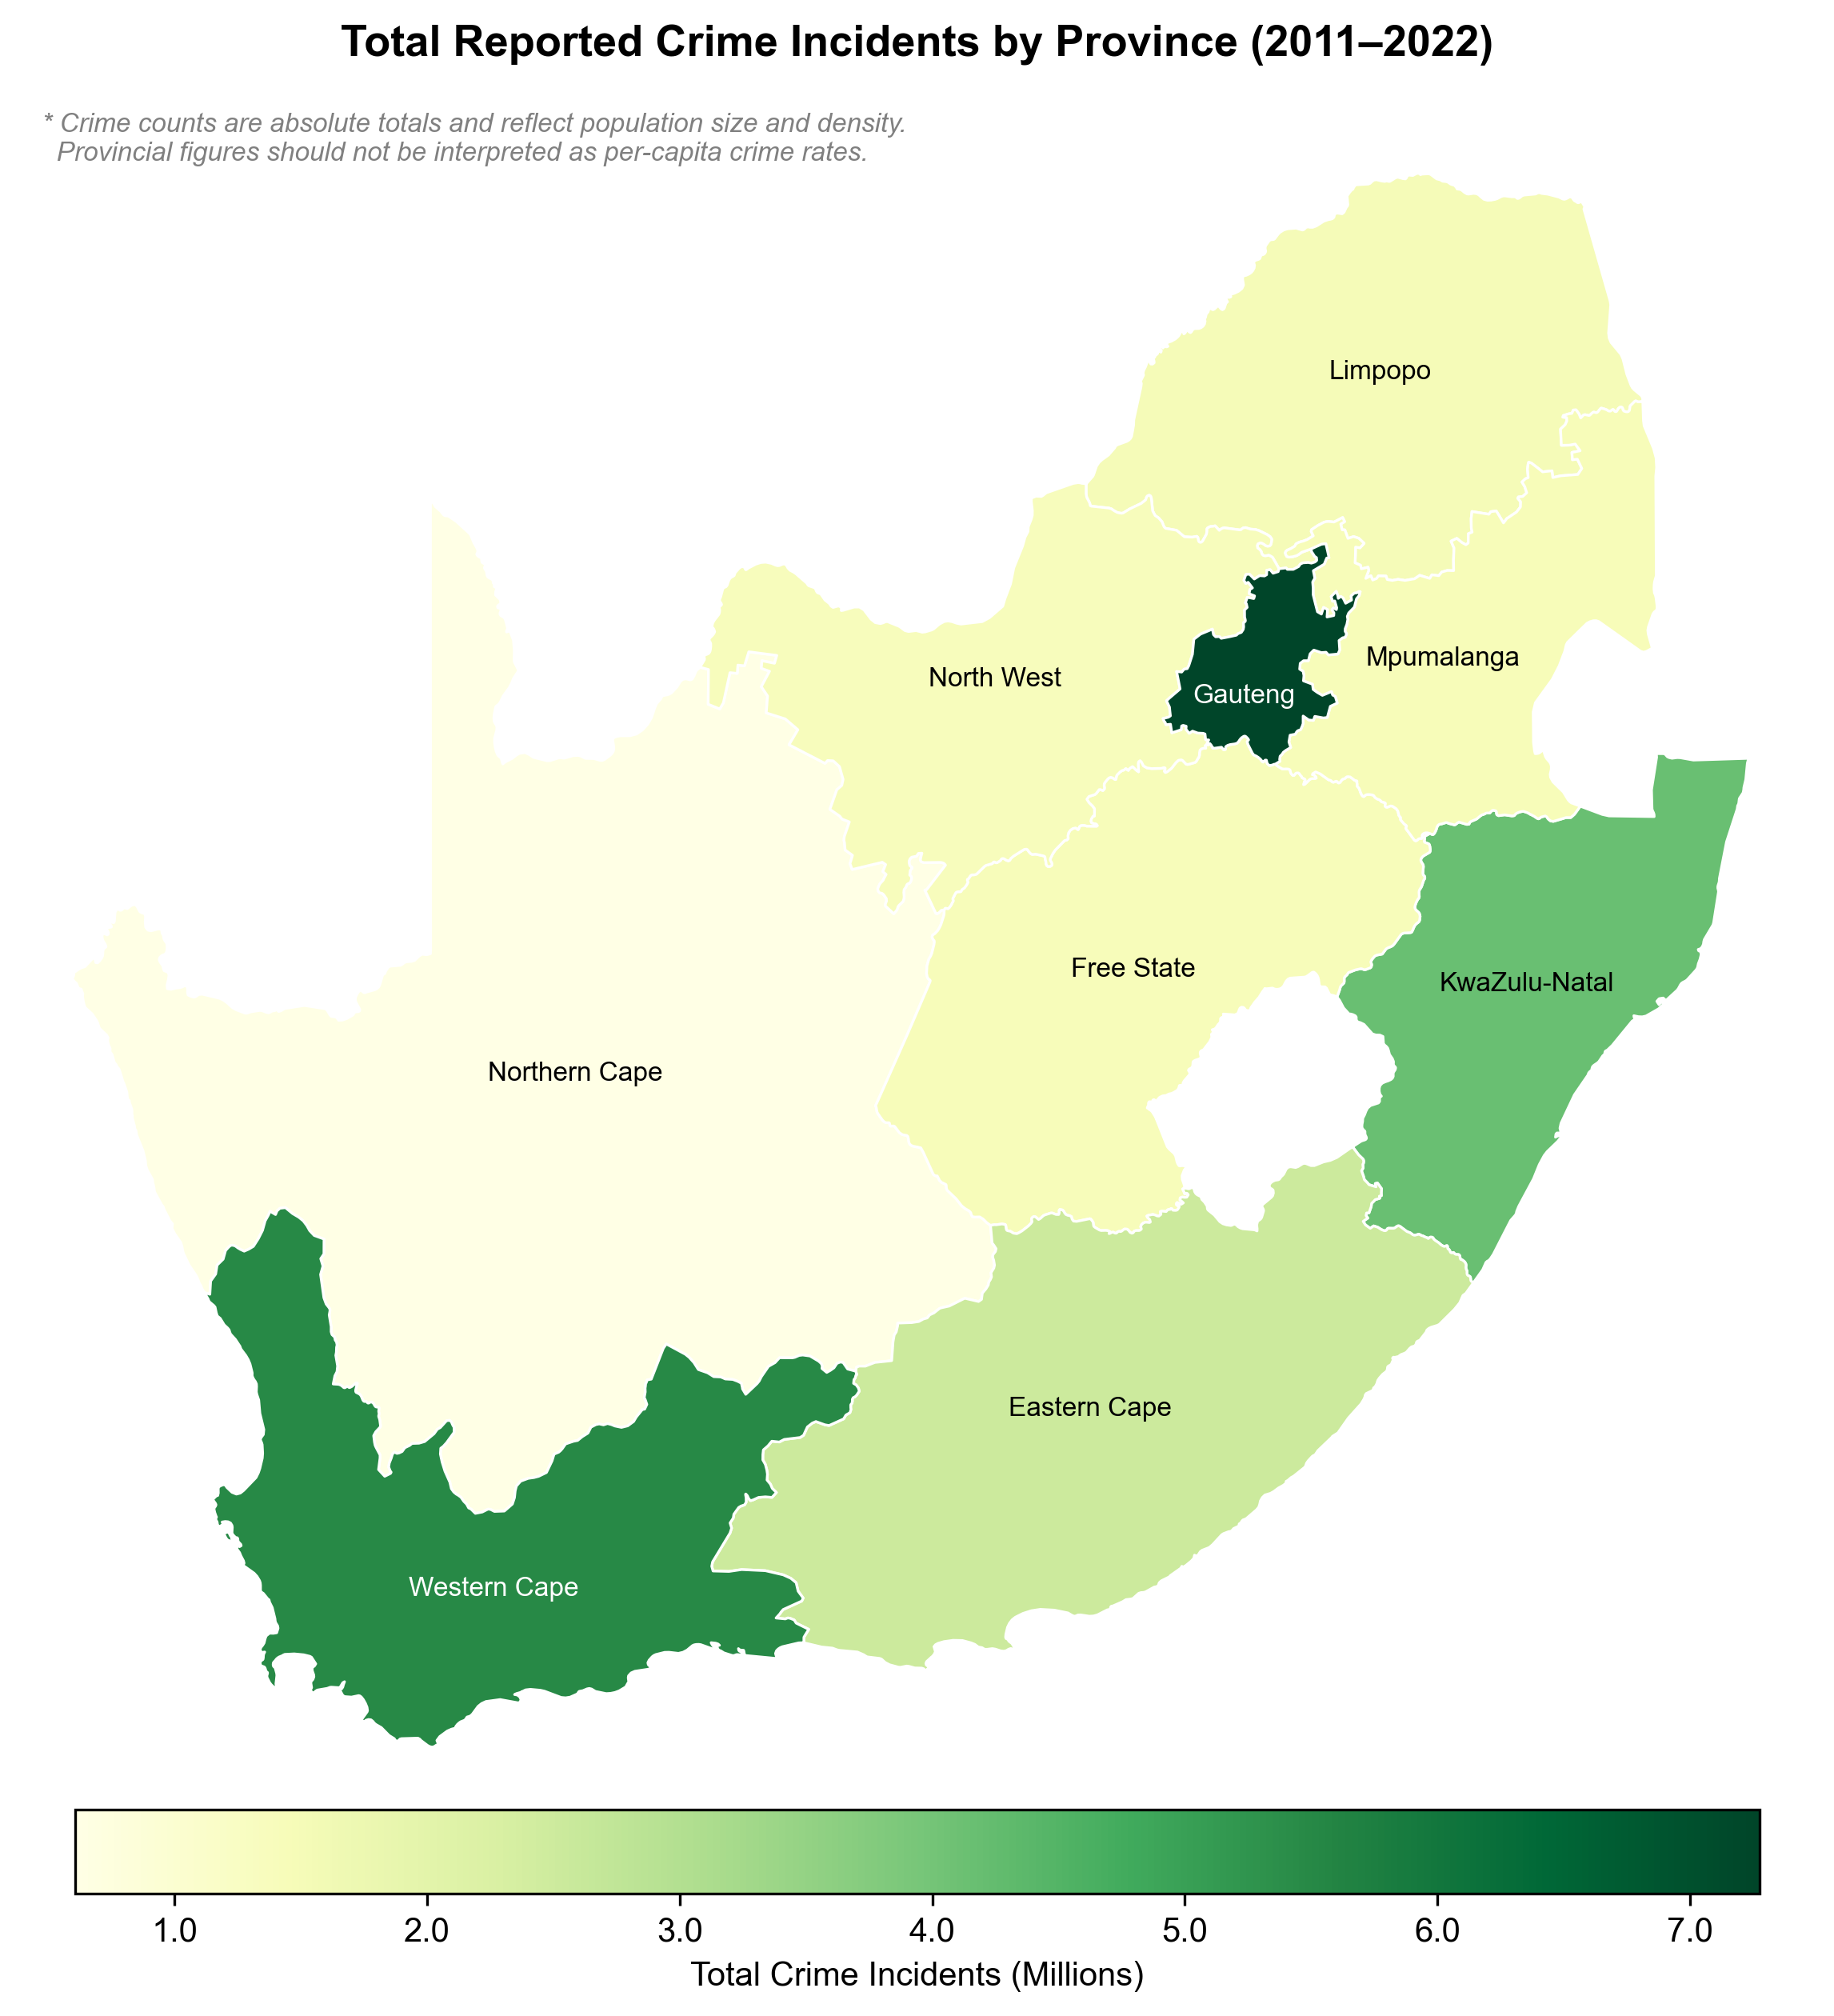
\includegraphics[width=0.825\linewidth]{choropleth_total.png}
	\caption{Cumulative provincial crime totals (2011 -- 2022).}
	\label{fig:choropleth_cumulative}
\end{figure}

\newpage

\section*{Trend Decomposition \& Forecasting}

\begin{figure}[H]
	\centering
	
\includegraphics[width=0.925\linewidth]{trend_analysis.png}
	\caption{Moving average trend decomposition for national contact crimes (2011 -- 2022).}
	\label{fig:trend_decomp}
\end{figure}

\vspace{\fill}

\begin{figure}[H]
	\centering
	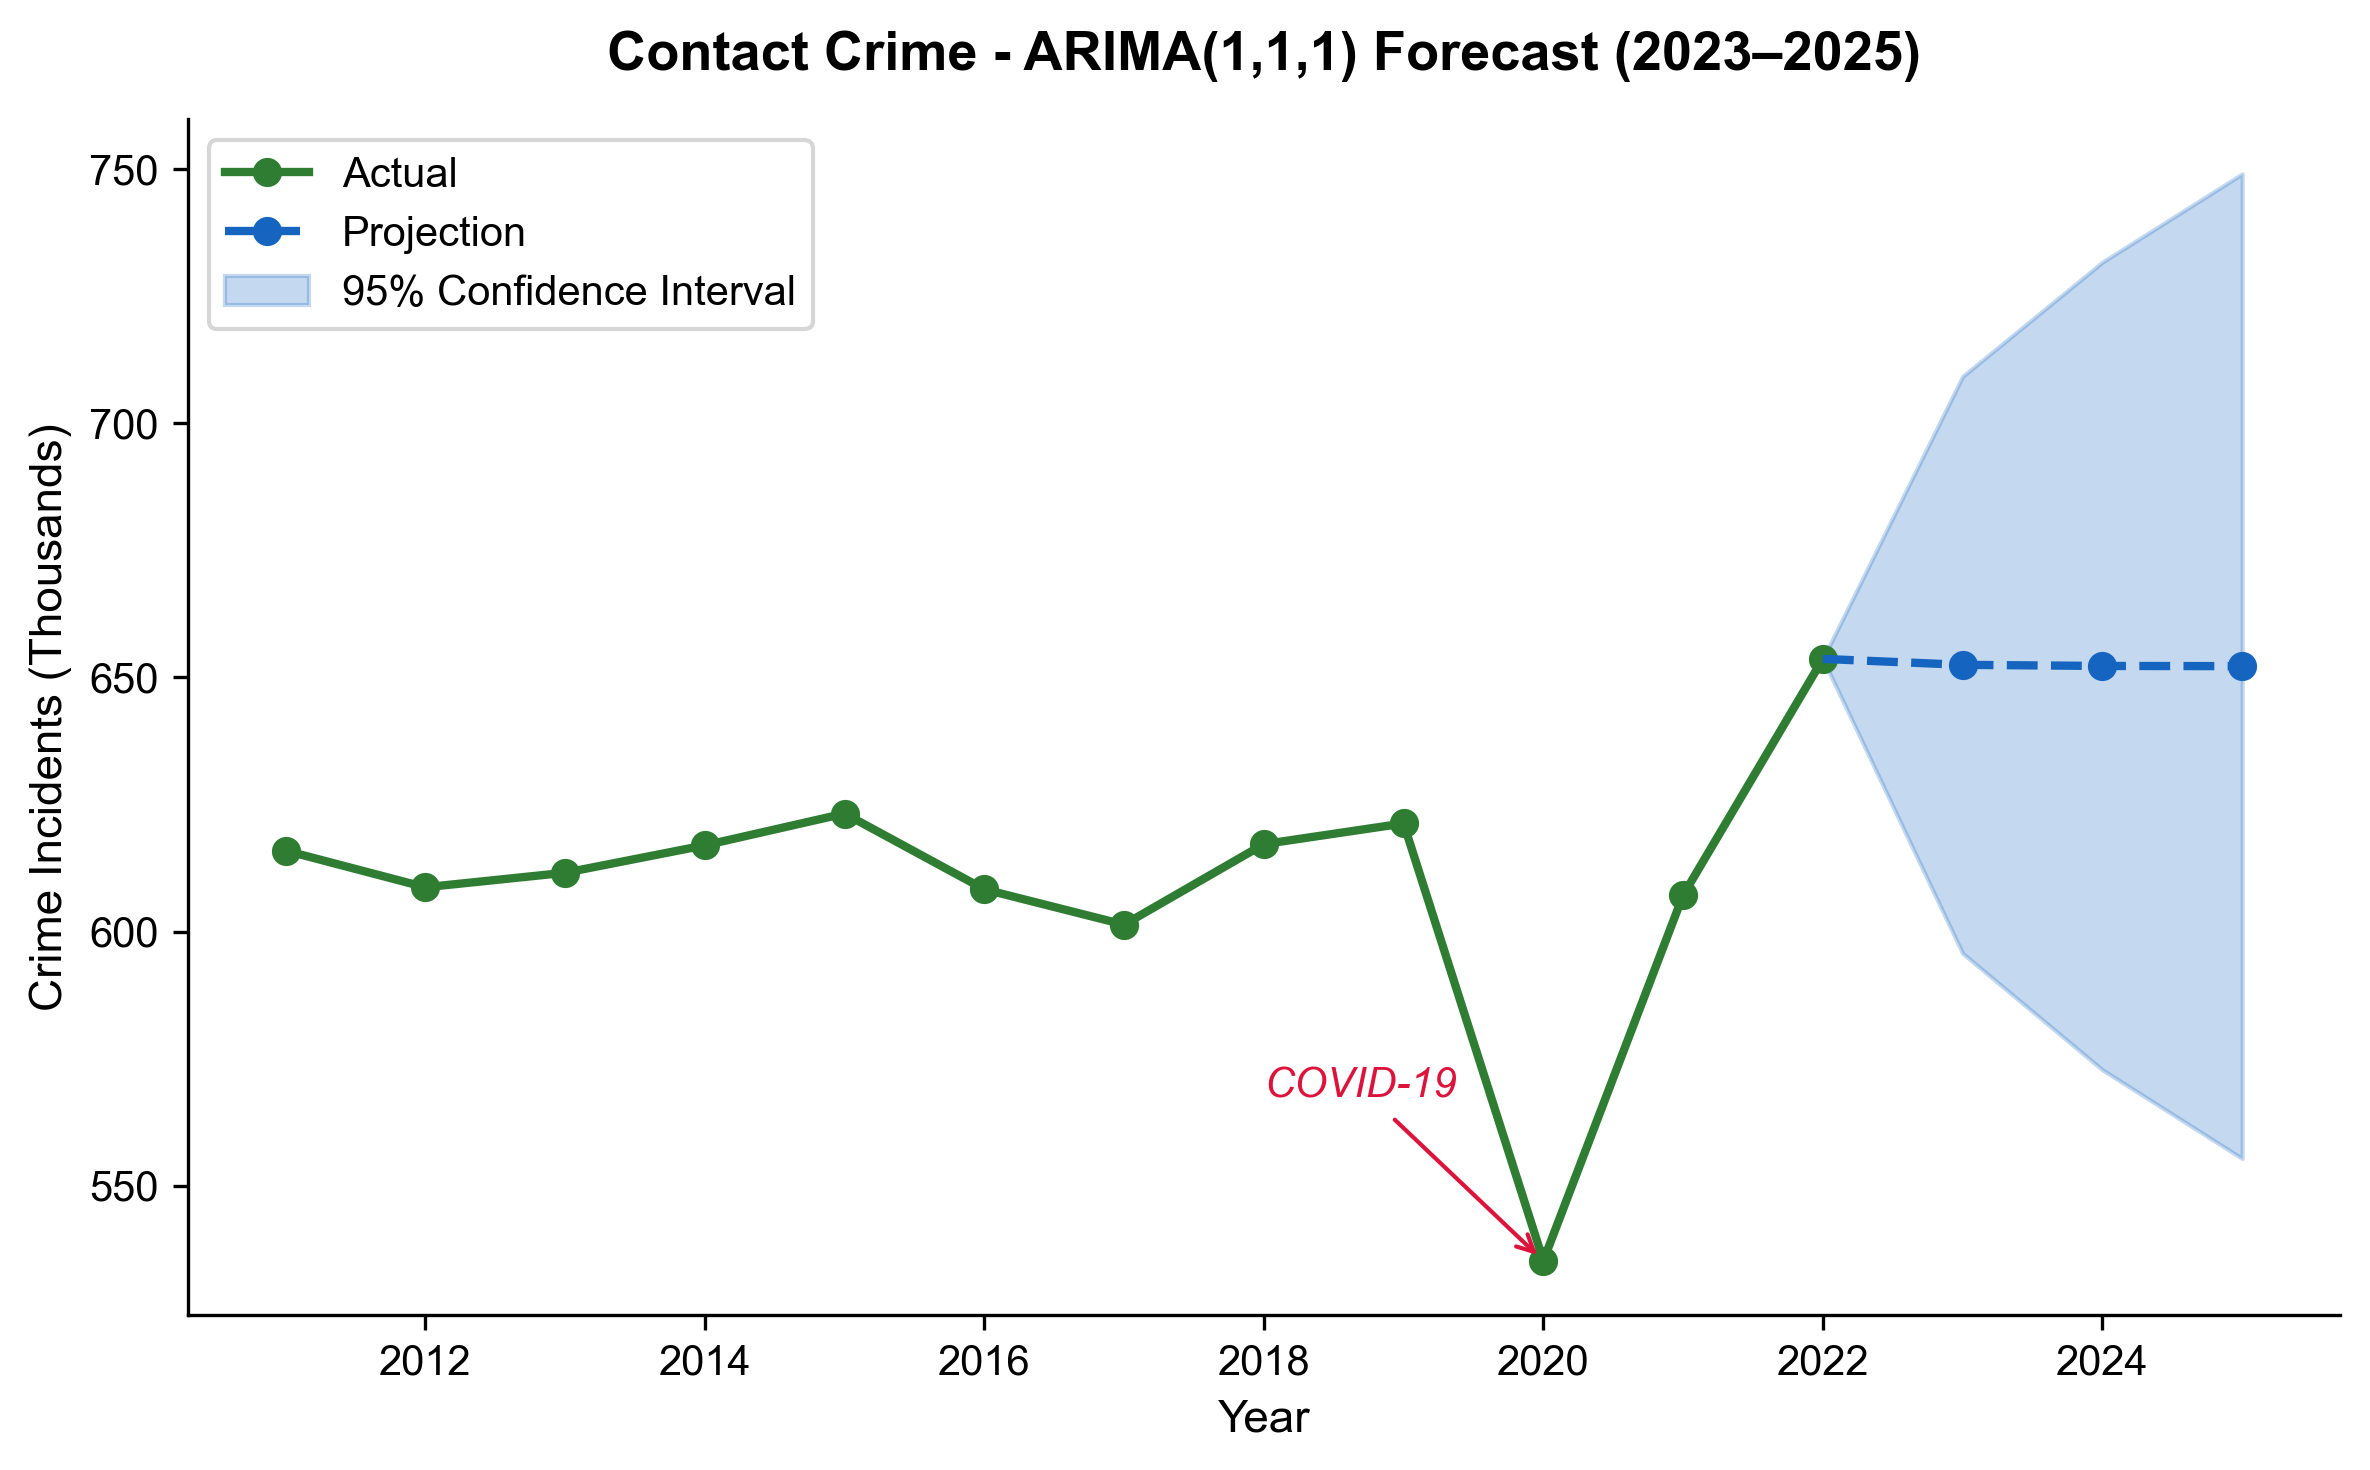
\includegraphics[width=0.925\linewidth]{forecast_chart.png}
	\caption{3-year forecast using \texttt{ARIMA(1,1,1)} for national contact crimes (2011 -- 2025).}
	\label{fig:forecast}
\end{figure}

\vspace{\fill}

\newpage

\section*{Key Findings \& Policy Implications}
\begin{tcolorbox}[
	colback=darkgreen!8!white,
	colframe=darkgreen,
	title={\textbf{Key Findings}},
	fonttitle=\bfseries,
	rounded corners,
	breakable]
	\begin{itemize}
		\item Gauteng, Western Cape and KwaZulu-Natal recorded the highest absolute crime totals across all years, revealing a structural geographic concentration of reported incidents reflective of urbanisation and population size.
		\item Community-reported incidents dominated the national crimescape, with contact crimes recording the highest absolute crime totals across all years. The top five categories shared two features: a 2020 minimum and post-lockdown rebound, reflective of the COVID-19 lockdown period and subsequent lifting of restrictions. Police action crimes experienced an increase across the 2011 – 2017 period, followed by a sharp decline post-2017 --- a reflection of
		policing intensity rather than genuine changes in criminal activity and public safety.
		\item The underlying pattern for national contact crimes comprised a broadly stable but slightly declining path for the 2011 – 2019 period, followed by a sharp rebound post-2020 --- confirmed the 2020 crime suppression to be temporary and not structural. The linear trend revealed that national contact crimes remained relatively stable across the full analysis period, indicating no long-term increase or decrease. 
		\item A nearly flat 3-year projection of national contact crime figures was produced for 2023 – 2025, with projected figures remaining close to the 2022 peak --- reflective of the sharp post-2020 rebound. The widening CI reflected the increased uncertainty from a short time series and COVID-19 anomaly. The nearly flat near-term projection suggests that, without any structural interventions, national contact crimes are unlikely to decline significantly from rebounded levels recorded in 2022.
	\end{itemize}
\end{tcolorbox}	

\noindent The key findings were relevant to several existing South African policing and safety frameworks, as they could potentially inform: (1) a data-driven approach for high-risk area crime targeting and allocation of policing resources, (2) the crime types and areas that may require priority-level intervention, (3) the annual resource allocation and operational planning at a national level, and (4) the planning of localised crime prevention initiatives and awareness campaigns through targeted crime operations.

\newpage

\section*{Limitations \& Conclusion}
Several limitations of the crime statistics and its findings were considered when results were interpreted:

\begin{itemize}
	\item The dataset contains absolute crime figures and not per-capita
	rates, meaning the figures reflect population size rather than individual crime risk.
	\item The dataset lacks police-station level crime figures. As such, sub-provincial spatial analysis was not possible.
	\item The 2020 crime figures were temporarily suppressed due to the national
	lockdown. Despite having been acknowledged as an anomaly throughout the analysis, the trend decomposition and forecast results may have been influenced by its presence in the time series.
	\item The \texttt{ARIMA(1,1,1)} was a simple model that was selected for
	interpretability and not precision. A more complex model or a longer
	time series would likely produce tighter confidence intervals and more reliable projections.
\end{itemize}

\noindent The purpose of this analysis was to answer four research questions concerning the spatial distribution, categorical composition, temporal patterns and short-term trajectory of the South African crimescape between 2011 and 2022. The analysis revealed: (1) the structural geographic concentration of crime in densely populated and urbanised provinces, (2) the dominance of serious community-reported crimes, with most categories being characterised by a general decline and a temporary COVID-19 anomaly, (3) the broadly stable underlying trend of national contact crimes, with no sustained long-term
increase or decrease, and (4) nearly flat near-term projection with no immediate
decline without structural intervention. This analysis demonstrates how publicly available structured crime data can reveal patterns not visible in annual headline figures. As such, the analysis can support existing strategic frameworks in an effort to tackle South Africa’s crime burden. \\\\
Several avenues exist for future work and a more advanced analysis. These include using population-normalised per-capita rates from Stats SA data, including station-level crime figures for sub-provincial spatial analysis, and using a more complex forecasting model for tighter near-term projections.
	
\end{document}